\documentclass[12pt]{beamer}

\usepackage[francais]{babel}
\usepackage[utf8]{inputenc}
\usepackage[T1]{fontenc}
\usepackage{multicol}
\usepackage{multirow}
\usepackage{graphicx} % Insertion d'images
\usepackage{amsmath}
\usepackage{tikz}

\graphicspath{{res/}}

\geometry{paperwidth=128mm,paperheight=110mm}
\usepackage[width=128mm,height=110mm,frame,noinfo]{crop}

\title{Management humain}
\author{Florian \bsc{Thuin}}
\institute{UCLouvain}
\date{\today}

\usetheme{Madrid}

\begin{document}
 \begin{frame}
  \titlepage
 \end{frame}
 
  \begin{frame}
    \frametitle{Management humain : de quoi parle-t-on ?}
    \fbox{\parbox{\linewidth}{
    \begin{multicols}{2}
	\centering \textbf{People Management}
	\centering Encadrement et leadership
	
	\begin{itemize}
	 \item Organisation et coordination du travail
	 \item Supervision et développement des individus
	 \item Aniamtion et conduite des équipes
	\end{itemize}
	
	\columnbreak
	
	\centering \textbf{Gestion des ressources humaines}
	
	\begin{itemize}
	 \item Recrutement et sélection
	 \item Allocation et planification
	 \item Classification et rémunération
	 \item Développement et formation
	 \item Evaluation des performances
	 \item Dialogue social, communication
	\end{itemize}

    \end{multicols}}}
    
    \centering $\Downarrow$
	
    Comportement manifestes et tacites individiuels et collectifs

  \end{frame}
  
  \begin{frame}
     \frametitle{Les niveaux d'intelligibilité d'Ardoino}
     
     \begin{figure}[!ht]
	\begin{center}
	    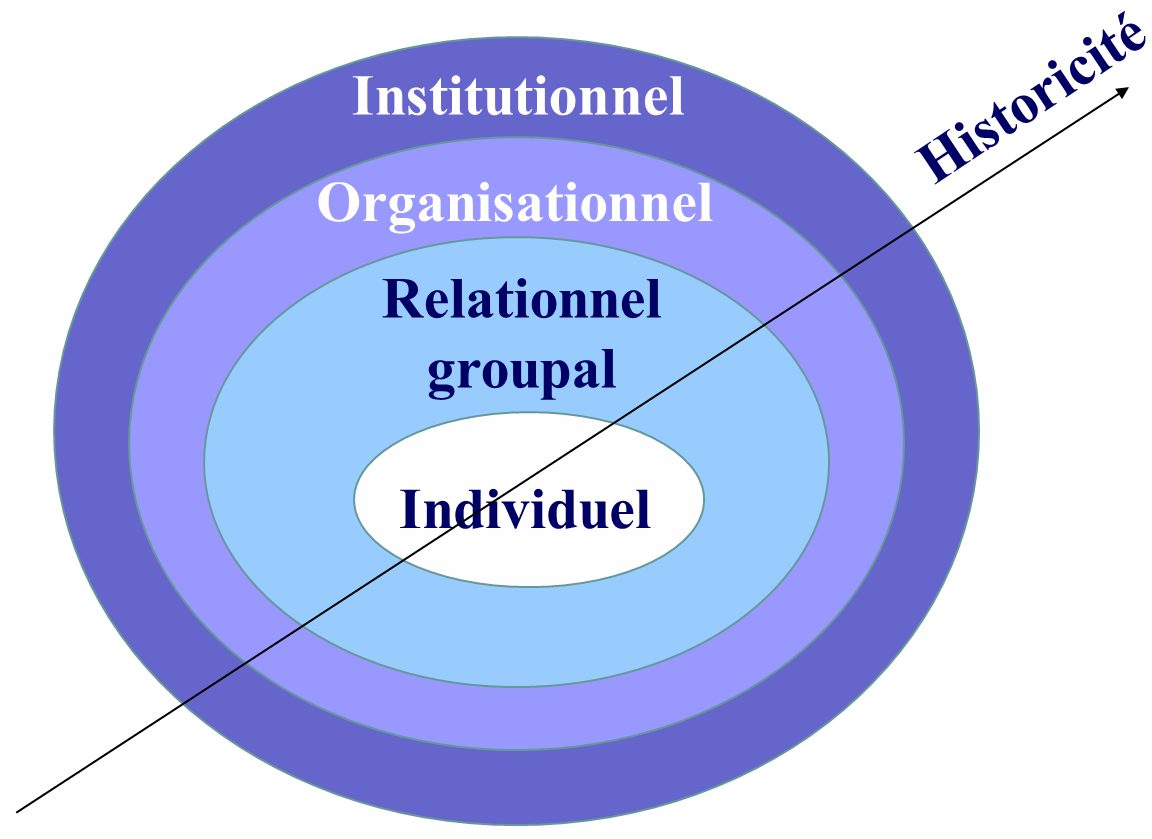
\includegraphics[scale=0.27]{niveaux_intelligibilite_ardoino.png}
	    \caption{Les niveaux d'intelligibilité d'Ardoino}
	\end{center}
     \end{figure}
     
  \end{frame}
  
  \begin{frame}[allowframebreaks]
      \frametitle{Les niveaux d'intelligibilité d'Ardoino}
      Selon Ardoino, 5 niveaux d'analyse et d'interprétation d'un phénomène social :
      
      \begin{enumerate}
       \item L'individuel
	    \begin{itemize}
	     \item facteurs individuels, souvent d'ordre psychologique (personnalité, motivations,...)
	     \item Niveau d'explication le plus spontanément invoqué, en raison de l'erreur fondamentale d'attribution
	    \end{itemize}
      \item Le relationnel et le groupal :
	  \begin{itemize}
	   \item Relation interpersonnelles et affectives, communication
	   \item Phénomènes de groupes : cohésion, appartenances, relations intergroupes
	  \end{itemize}
      \item L'organisationnel
	  \begin{itemize}
	   \item Modalités d'organisation de l'action collective : règles, rôles, statuts, modes de division et de coordination du travail, structures de pouvoir et allocation des ressources
	  \end{itemize}
      \framebreak
      \item L'institutionnel :
	  \begin{itemize}
	   \item Institutions publiques, cadres politique, juridique, social, économique dans lesquels les organisations évoluent
	   \item Règles formelles (lois, codes, règlements) et informelles (cultures, valeurs, traditions et conventions) qui régissent l'ensemble de la société
	  \end{itemize}
      \item L'historicité
	  \begin{itemize}
	   \item Transformations de la société, mouvements sociaux, tendances économiques
	   \item Jeux des rapports de force entre acteurs et classes sociales qui président à la transformation de la société
	  \end{itemize}

      \end{enumerate}
  \end{frame}
    
  \begin{frame}
    \frametitle{Le modèle de Kolb}
	\underline{Le modèle de Kolb présente un cycle d'apprentissage expérientiel :}
	
	\begin{figure}[!ht]
	    \begin{center}
		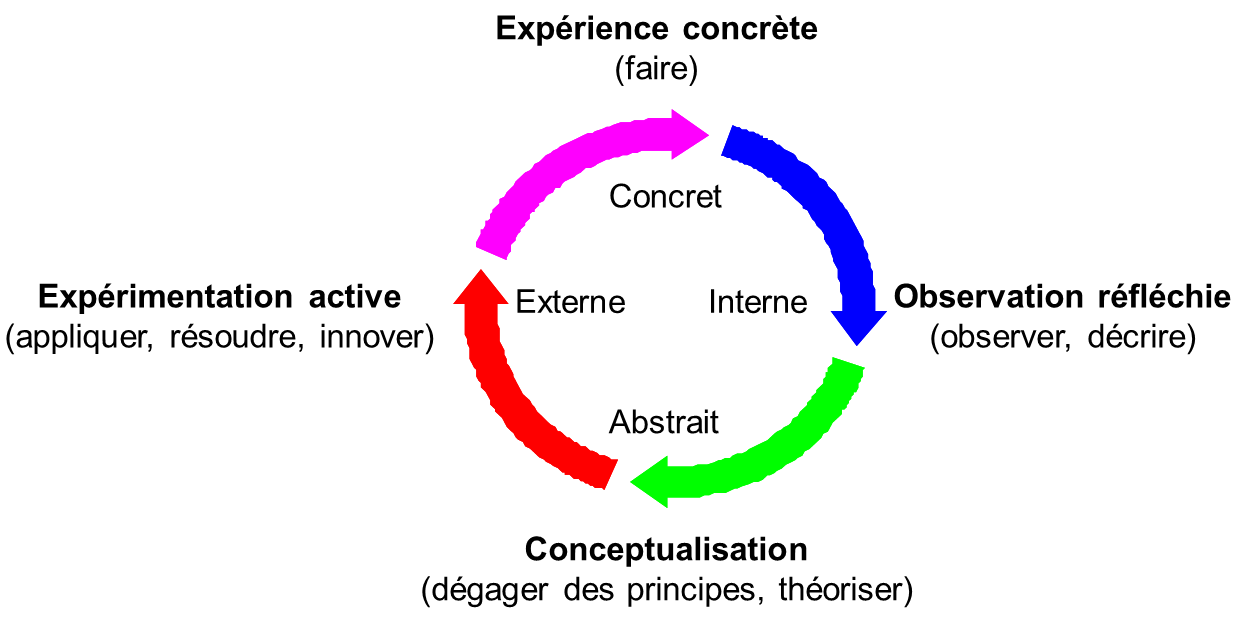
\includegraphics[scale=0.25]{modele_de_kolb.png}
	    \end{center}
	\end{figure}
  \end{frame}

\section{Histoire de la GRH}
  \begin{frame}
      \frametitle{La gestion des ressources humaines comme construction historique}
      \textit{De l'administration du personnel à la gestion stratégique des ressources humaines}
      \bigskip
      
      4 étapes historiques :
      
      \begin{itemize}
       \item 4 contextes socio-économiques distincts
       \item 4 modèles dominants d'organisation du travail et de pensée stratégique
       \item 4 conceptions sous-jacentes de l'être humain
       \item 4 rôles distincts pour la fonction RH
      \end{itemize}
      
  \end{frame}
  
  \begin{frame}
    \frametitle{Les 4 rôles RH (Ulrich, 1993)}
	\begin{tabular}{cp{4.8cm}|p{4.8cm}c}
	& \multicolumn{2}{c}{Personnes} & \\
	\hline
	 \multirow{2}{2mm}{\rotatebox{90}{Opérationnel}} & \textbf{\underline{Champion des employés}} : assurer que les membres du personnel fassent ce qui est attendu d'eux, y trouvent satisfaction, puissent se développer et restent impliqués & \textbf{\underline{Agent de changement}} : assurer que la culture de l'organisation évolue de sorte que le comportements des individus soient bien adaptés à l'environnement & \multirow{2}{2mm}{\rotatebox{270}{Stratégique}} \\
	 \hline
	  & \textbf{\underline{Expert administratif}} assurer que les règles, processus, systèmes et outils RH fonctionnent de manière efficace et efficiente  & \textbf{\underline{Partenaire stratégique}} : assurer que le déploiement des ressources humaines aide l'organisation à atteindre ses objectifs & \\
	  \hline
	& \multicolumn{2}{c}{Processus} & \multicolumn{1}{l}{} \\      
	\end{tabular}
  \end{frame}
  
  \begin{frame}
      \frametitle{Contexte socio-économique}
      La première étape est la \textbf{révolution industrielle} :
      
      \begin{itemize}
       \item Progrès technologique : machinisme
       \item Industrialisation massive de la production
       \item Disparition des corporations de métiers
       \item Arbitraire, prfs paternaliste, du patron
       \item Avènement de l'entreprise capitaliste
       \item Construction d'un marché de libre échange
       \item Naissance des valeurs démocratiques républicaines
      \end{itemize}
  \end{frame}
  
  \begin{frame}
    \frametitle{Contexte socio-économique}
    
    $\Rightarrow$ \textbf{La dualisation de la société} :
    \begin{center} bourgeoisie industrielle VS prolétariat \end{center}
    
    $\Rightarrow$ Perte d'autonomie et \textbf{déqualification progressive} des travailleurs
    
    $\Rightarrow$ Conditions de travail misérables et \textbf{précarisation économique} de la classe ouvrière
    
    $\Rightarrow$ \textbf{Naissance du mouvement ouvrier} et du syndicalisme
    \begin{center} $\Rightarrow$ législation sociale et concertation sociale \end{center}
    
  \end{frame}
  
  \begin{frame}
      \frametitle{Modèles d'organisation du travail}
      
      \textbf{Organisation scientifique du travail} (Taylorisme) :
      
      \begin{itemize}
       \item Standardisation : parcellisation et simplification des tâches (chronométrage des temps et mouvements)
       \item Distinction conception-exécution
      \end{itemize}
      
      \textbf{Bureaucratie wébérienne} :
      
      \begin{itemize}
       \item Formalisation et impersionnalité : la règle remplace la tradition et l'arbitraire
       \item Centralisation et hiérarchisation : structure hiérarchique conforme au principe d'unité de commandement
      \end{itemize}
      
      \textbf{Fordisme} :
      
      \begin{itemize} \item gains productivité et croissance assurés par une production et une consommation de masse \end{itemize}
      
      \textbf{Planification rationnelle} (One best way) :
      
      \begin{itemize} \item dans un environnement stable et peu compétitif \end{itemize}
      
  \end{frame}
  
  \begin{frame}
    \frametitle{Conception de l'homme}
    
    \begin{itemize}
     \item \textbf{Main-d'oeuvre} vite opérationnelle et substituable
     \item Dominance du \textbf{courant behavioriste} en psychologique industrielle
     \item Postulat de \textbf{l'homme économique} :
	\begin{itemize}
	 \item être paresseux attiré par les stimulants monétaires
	 \item être irresponsable dont il faut organiser, planifier, contrôler le travail
	\end{itemize}
    \item Forme d'intégration : \textbf{engagement calculé}, fondé sur des incitiations extrinsèques
    \end{itemize}
  \end{frame}
  
  \begin{frame}
    \frametitle{Conception de la fonction RH}
    
    \textbf{Expert administratif} (D. Ulrich) \og{} bureau du personnel \fg{}
    
    \begin{itemize}
     \item Admnistration des contrats de travail
     \item Conception des systèmes de contrôle formelles
     \item Elaboration des systèmes de rémunération/incitation et gestion de la paie
     \item Prévention et gestion des conflits sociaux
     \item Profil du \og{} DRH \fg{} : l'ingénieur, puis le juriste
    \end{itemize}
  \end{frame}
  
  \begin{frame}
    \frametitle{Pratiques héritées en RH}
    
    \begin{itemize}
     \item \textbf{Analyse du travail} et description de poste
     \item Développement de la \textbf{concertation sociale} en réponse au mouvement ouvrier et au syndicalisme
     \item \textbf{Classification des emplois et barèmes salariaux}
     \item \textbf{Sécurité physique et hygiène}
    \end{itemize}
  \end{frame}
  
  \begin{frame}
    \frametitle{Historique de la concertatioon sociale en Belgique}
    
    \begin{center} \textbf{1850 à 1900 : Naissance du mouvement ouvrier et du syndicalisme} \end{center}
    
    \begin{itemize}
     \item 1858 : Création à Gand du premier syndicat dans le textile
     \item 1866 : Abrogation de l'interdiction de coalition qui permet le développement des syndicats
     \item 1886 : Grèves et émeutes en Wallonie, fortement réprimées par l'Etat
    \end{itemize}
    
    $\Rightarrow$ Institution des conseils de l'industrie et du travail (1887)
    
    $\Rightarrow$  Limitation du travail des femmes et des enfants (1889)
    
    $\Rightarrow$ Suffrage universel et pluraliste (1893)
  \end{frame}
  
  \begin{frame}
    \frametitle{Historique de la concertation sociale en Belgique}
    
    \textbf{1900 à 1945 : Fédérations des mouvements syndicaux et institutionnalisation des organes de la concertation sociale}
    
    \begin{itemize}
     \item 1895 : Création du Comité central du travail industriel, première organisation patronale nationale
     \item Fédérations des syndicats : CSC (1912), CGSLB (1930), FGTB (1945) 
     \item 1919 : Premières commissions paritaires dans les mines, la sidérurgie et les constructions mécaniques
     \item 1921 : Liberté syndicale garantie à travers la reconnaissance de la liberté d'association et l'abrogation de l'interdicition du droit de grève
     \item 1936 : 500.000 travailleurs en grève
    \end{itemize}
    
    $\Rightarrow$ première conférence nationale du travail : 1 semaine de congé payé, semaine de 40 heures dans les mines, salaire minimum garanti et augmentation des allocations familiales
  \end{frame}
  
  \begin{frame}
    \begin{center} \textbf{1944 à 1975 : Pacte social} \end{center}
    
    1944 : Conclusion du Projet d'accord de solidarité sociale - 3 conceptions sous-jacentes (P. Reman, CRISP, 2010)
    
    \begin{description}
     \item[Progrès : ] \og{} Le progrès social découle à la fois de l'essor économique d'un monde pacifié et d'une équitable répartition du revenu d'une production croissante. \fg{}
     \item[Concertation : ] \og{} Les relations entre employeurs et travailleurs doivent être fondées sur le respect mutuel et la reconnaissance réciproque de leurs droits et devoirs \fg{}
     \item[Protection sociale : ] \og{} l'assurance maladie-invalidité et l'assurance chômage deviennent obligatoires, sont financées par une cotisation prélevée sur les salaires et sont gérées paritairement. \fg{} (Modèle bismarckien)
    \end{description}
  \end{frame}
  
  \begin{frame}
    \frametitle{Historique de la concertation sociale en Belgique}
    \begin{center} \textbf{1944 à 1975 : Pacte social} \end{center}
    
    $\Rightarrow$ \textbf{Construction du système actuel de concertation sociale :}
    
    Mise en place des commissions paritaires (1945), des délégations syndicales (1947), du conseil central de l'économie et des conseils d'entreprise (1948), du Conseil national du travail et des comités de sécurité et d'hygiène (1952)
    
    $\Rightarrow$ \textbf{Accords interprofessionnels et conventions collectives de travail améliorant les conditions de travail}
    
    p. ex. : négociation des barèmes salariaux, indexation automatique des salaires, augmentation des congés payés, généralisation de la journée de 8 heures et de la semaine de 40 heures
    
    $\Rightarrow$ \textbf{Développement de la sécurité sociale} sur un principe de solidarité et de répartition des revenus :
    
    pensions, allocations chômage et incapacité de travail, couverture soins de santé, allocations familiales, crédit temps, congé éducation,...
    
  \end{frame}
  
  \begin{frame}
    \frametitle{Les acteurs de la concertation en Belgique}
    
    \begin{itemize}
     \item Syndicats :
	\begin{itemize}
	 \item Confédération des Syndicats Chrétiens (CSC)
	 \item Fédération Générale du Travail de Belgique (FGTB)
	 \item Confédération Générale des Syndicats Libéraux de Belgique (CGSLB)
	 \item Confédération Nationale des Cadres (CNC)
	\end{itemize}
	
     \item Patronat :
	\begin{itemize}
	 \item Fédération des Entreprises de Belgique (FEB)
	 \item Union des Classes Moyennes (UCM - UNIZO)
	 \item Organisations agricoles
	\end{itemize}
    \end{itemize}
  \end{frame}
  
  \begin{frame}
    \frametitle{Les instances de la concertation sociale en Belgique}
    
    \begin{tikzpicture}
      \tikzstyle{ellypse}=[circle, draw, fill=blue!50, text=black]
      \tikzstyle{rectangle}=[draw, thick, fill=red!50]
      \tikzstyle{fleche}=[->,>=latex,thick]
      
      \node[rectangle] (Dir) at (-2,0) {Direction};
      \node[ellypse, text width=3.5cm] (Cons) at (2.5,2.5) {\textbf{Conseil d'entreprise} (à partir de 100 travailleurs)};
      \node[ellypse, text width=3.5cm] (Comi) at (2.5,-2.5) {\textbf{Comité pour la Prévention et la Protection au Travail} (à partir de 50 travailleurs)};
      \node[rectangle] (Del) at (7,0) {Délégation syndicale};
      \node[text width=3.5cm] (Elec) at (7.5,-3) {Elections sociales (tous les 4 ans)};
      \node[text width=4cm] (Reg) at (7.5, 3) {Règlement de travail};
      \draw[fleche] (Dir)--(Cons);
      \draw[fleche] (Dir)--(Comi);
      \draw[fleche] (Del)--(Cons);
      \draw[fleche] (Del)--(Comi);
      \draw[fleche] (Elec)--(Del);
      \draw[fleche] (Cons)--(Reg);
      
    \end{tikzpicture}
  \end{frame}
  
  \begin{frame}
    \frametitle{Les instances de la concertation sociale en Belgique}
    
    \textbf{Au niveau des catégories socio-professionnelles et secteurs d'activités :}
    
    \begin{tikzpicture}
      \tikzstyle{ellypse}=[circle, draw, fill=blue!50, text=black]
      \tikzstyle{rectangle}=[draw, thick, fill=red!50]
      \tikzstyle{fleche}=[->,>=latex,thick]
      
      \node[rectangle, text width=3cm] (Pat) at (-2,0) {Organisations patronales};
      \node[ellypse, text width=3.5cm] (Comm) at (2.5,0) {\textbf{Commissions paritaires} (94 commissions et 74 sous-commissions)};
      \node[rectangle, text width=3cm] (Synd) at (7,0) {Organisations syndicales};
      \node (Conv) at (2.5,-3.5) {Conventions collectives de travail};
      \draw[fleche] (Pat)--(Comm);
      \draw[fleche] (Synd)--(Comm);
      \draw[fleche] (Comm)--(Conv);
      
    \end{tikzpicture}
  \end{frame}
  
  \begin{frame}
    \frametitle{Les instances de la concertation sociale en Belgique}
    
    \textbf{Au niveau interprofessionnel :}
    
    \begin{tikzpicture}
      \tikzstyle{ellypse}=[circle, draw, fill=blue!50, text=black]
      \tikzstyle{rectangle}=[draw, thick, fill=red!50]
      \tikzstyle{fleche}=[->,>=latex,thick]
      
      \node[rectangle, text width=3.2cm] (FEB) at (-2,0) {FEB (8 mandats) UCM/UNIZO (3) UPA/Boerenbond (1)};
      \node[ellypse, text width=2.5cm] (Econ) at (2.5,2.5) {\textbf{Conseil Central de l'Economie}};
      \node[ellypse, text width=2.5cm] (Trav) at (2.5,-1) {\textbf{Conseil National du Travail}};
      \node[rectangle, text width=2cm] (CSC) at (7,0) {CSC (6) FGTB (5) CGSLB(1)};
      \node[text width=6cm] (Conv) at (2.5,-3.5) {Conventions collectives de travail + Accords interprofessionels};
      \draw[fleche] (FEB)--(Trav);
      \draw[fleche] (CSC)--(Trav);
      \draw[fleche] (Econ)--(Trav);
      \draw[fleche] (Trav)--(Conv);
      
    \end{tikzpicture}
    
  \end{frame}
  
  
  
 \begin{frame}
    \frametitle{Un exemple de titre}
      \framesubtitle{Exemple de sous-titre}
 \end{frame}
 
 \begin{frame}[plain]
  Pas d'en-tête ou pied de page.
 \end{frame}

\end{document}
